
\documentclass{article}

\usepackage[ngerman]{babel}                     %for german umlauts
\usepackage[utf8]{inputenc}
\usepackage{subfigure}
\usepackage{float}
%\usepackage[framed,autolinebreaks,useliterate]{mcode}
%\usepackage[bw,framed,autolinebreaks,useliterate]{mcode}
% \usepackage[ansinew]{inputenc}        %for german umlauts

\usepackage{listings}

\usepackage{graphicx}
\usepackage{hyperref}

\usepackage{amssymb}    %for different fonts
\usepackage{amsmath}
% Geht nicht: \usepackage{bbm}
% \usepackage[usenames,dvips]{color} %only way to get it running with pdf:(
% \usepackage[pdftex,usenames,dvipsnames]{color}        % does not work
% \usepackage{color}
\usepackage{verbatim}
\usepackage{polynom}

\setlength{\parindent}{0pt}
\addtolength{\hoffset}{-2cm}
\addtolength{\voffset}{-1cm}
\addtolength{\textheight}{3cm}
\addtolength{\textwidth}{3cm}

\newcommand{\im}{\operatorname{Im}}
\newcommand{\rg}{\operatorname{rg}}
\newcommand{\ggt}{\operatorname{ggT}}

\lstset{ %
  language=Matlab,                % the language of the code
  frame=single,                   % adds a frame around the code
  tabsize=2,
  basicstyle=\footnotesize
}

\begin{document}

\section*{\begin{center} Mustererkennung - Aufgabenblatt 07 \end{center}}
\begin{center}
  André Hacker und Dimitri Schachmann \\
\end{center}


\subsection*{0. Backpropagation Algorithmus}
Für beiden Aufgaben haben wir die gleiche Implementierung des
Backpropagation Algorithmus verwendet, weswegen wir sie hier erstmal
gesondert vorstellen.\\

Wir verwenden Online Learning und wählen den Input in jeder Iteration zufällig.\\

Um besser abzuschätzen, wie gut der Algorithmus tatsächlich in jeder Iteration für alle Samples 
funktioniert, berechnen wir zusätzlich den Fehler für alle Samples.
Über den Parameter errorEvery kann man steuern, dass der globale Fehler
nicht in jeder Iteration berechnet wird (zeitaufwändig).\\

Die Ausgabe Y (bisher immer skalarer Wert von 0 bis 9) musste vorab in eine Dummy-Variablen Darstellung überführt werden.
Die Klasse 2 entspricht dann der Variable $ (0, 0, 1, 0, 0, 0, 0, 0, 0, 0) $.

\begin{lstlisting}
% Learns the weights of a 2 Layer Neural Network
% Uses Online (sequential) Training
% @param X: Samples
% @param Y: Output (encoded as dummy variables)
% @param K: Number of hidden nodes
% @param M: Number of output nodes
% @param learnFactor: Learning rate
% @param maxIterations: when to stop
% @param errEvery: Error (for all items) will be calculated only every ... iterations.
%                  Error computation is very costly, so we don't want to do it in every step
% 
% @return W1d: weights of the 1st layer
%
% @return W2d: weights of the 2nd layer
%
% @return Eabs: Matrix. Eabs(i,j) is the absolute avarage deviation
% (abs(predicted - y)) for the j-th output unit in iteration i. For
% all samples
%
% @return Esq: Matrix. Esq(i,j) is the half squared avarage deviation
% (((predicted - y)^2)/2) for the j-th output unit in iteration i. For
% all samples
%
% @return Eonline: column vector. Eonline(i) is the the half
% squared error for the current random sample in iteration i of
% online learning. That is the function that we optimize for.
  function [W1d W2d Eabs Esq Eonline] = learnNeural(X, Y, K, M, learnFactor, ...
  	maxIterations, errEvery)
  
  D = size(X, 2);   % number of input nodes (dimensionality of input)
  N = size(X, 1);   % number of input items
  Xd = [X, ones(size(X, 1), 1)];  % convenience

  % Track global (for all training items) absolute deviation for each output unit
  Eabs = zeros(ceil(maxIterations/errEvery), M); 
  Esq = zeros(ceil(maxIterations/errEvery), M);
  Eonline = zeros(maxIterations, 1);

  % Start with random initial weights
  % 1st col = all weights to 1st node
  W1 = rand(D, K)*2-1;  % from -1 to 1
  W2 = rand(K, M)*2-1;
  W1d = [W1; rand(1, K)];
  W2d = [W2; rand(1, M)];
  if false
    W1 = ones(D, K);  % from -1 to 1
    W2 = ones(K, M);
    W1d = [W1; ones(1, K)];
    W2d = [W2; ones(1, M)];
  end
  
  for i=1:maxIterations
    % 0) Pick random input vector for online learning
    id = randi(size(X,1));
    x = X(id, :);
    xd = Xd(id, :);
    y = Y(id, :);
    
    % 1) Forward Propagation:
    % 1.1) Compute Layer hidden layer output o1
    % and Output layer output o2
    o1 = sigmoid(xd*W1d);   % 1xK
    o1d = [o1 1];
    o2 = sigmoid(o1d*W2d);  % 1xM
    o2d = [o2 1];
    
    % 1.2) Compute Derivations for Hidden units (D1)
    % and Output Units (D2) (diagonal matrix)
    D1 = diag(o1.*(1-o1));   % KxK
    D2 = diag(o2.*(1-o2));   % MxM
    
    % 1.3) Compute Derivation DE for Error unit
    DE = (o2-y)';  % Mx1

    Eonline(i) = sum((DE.^2)/2)/M;

    % Error-Tracking
    if (mod(i-1, errEvery) == 0)
      tmp=zeros(N, M);
      for l=1:N
        tmp(l,:) = evalNetwork(W1d, W2d, Xd(l,:));
      end
      Eabs((i-1)/errEvery+1, :) = sum(abs(tmp - Y), 1);
      Esq((i-1)/errEvery+1, :) = sum(((tmp - Y).^2),1) / 2;
    end

    % 2) Back Propagation
    % to Output Layer
    backErr2 = D2*DE;
    % to Hidden Layerm
    backErr1 = D1 * W2 * backErr2;
    
    % 3) Compute weight adoptions and adopt weights
    DeltaW2d = (-learnFactor * backErr2 * o1d)';
    DeltaW1d = (-learnFactor * backErr1 * xd)';
    W2d = W2d + DeltaW2d;
    W1d = W1d + DeltaW1d;
    W2 = W2d(1:end-1,:);
    W1 = W1d(1:end-1,:);
  end
end


% Logistic sigmoid function
function r = sigmoid(x)
  r = 1./(1 + exp(-x));
end

% Standardize data by subtracting the mean and deviding by the standard
% deviation
function r = standardize(samples)
  m = mean(samples);
  sd = std(samples);
  for i = 1:size(samples,1)
    samples(i,:) = (samples(i,:) - m) ./ sd;
  end
  r = samples;
end

% trasform data to a new basis, given by eigenspace (eigenvectors)
function r = transformData(eigenspace, data, dim)
  r = (eigenspace(:,end-dim+1:end)'*data')';
end

% computes the principal components for the given data
% r = eigenvectors of the covariance matrix
function r = principalComponents(data)
  covarMatrix = cov(data);
  [r eigen_values] = eig(covarMatrix);
end

% Plot Error rate over iterations
function plotErrorForIterations(E, name, xtitle, ytitle)
  h = figure();
  hold on;
  xlabel(xtitle, 'FontSize', 15);
  ylabel(ytitle, 'FontSize', 15);
  for i=2:(size(E,2))
    plot(E(:,1),E(:,i));
  end
  print(h,'-deps',[name '.eps']);
end

\end{lstlisting}
\subsection*{1. XOR}
Für diese Aufgabe sollte die XOR Funktion mit einem speziellen neuronalen Netz gelernt werden. Wir haben dafür einfach unsere generische Backpropagation Implementierung learnNeural aufgerufen (siehe oben).
Zum Vergleich haben wir auch OR und AND gelernt, was wesentlich schneller ging, vermutlich da diese linear separierbar sind.\\
\begin{lstlisting}
function xor()
  K = 2;  % number of hidden nodes
  M = 1;  % number of output nodes
  learnFactor = 1;  % Learning rate
  maxIterations = 20000;
  X = [0 0; 0 1; 1 0; 1 1]; % input samples (named o in book)
  YXOR = [0; 1; 1; 0];  % XOR
  YAND = [0; 0; 0; 1];  % AND
  YOR = [0; 1; 1; 1];  % OR
  [W1d W2d Eabs Esq Eonline] = learnNeural(X, YXOR, K, M, ...
      learnFactor, maxIterations, 1);
  plotErrorForIterations([[1:size(Eabs,1)]' Eabs./4], 'task1-xor-error', ...
      'Iterations','Mean Absolute Error');  %sum absolute error
  Dev = Eabs(end,:)
  meanDev = Eabs(end,:) / 4

  % Test output for generated weights
  res00 = evalNetwork(W1d, W2d, [0 0 1])
  res01 = evalNetwork(W1d, W2d, [0 1 1])
  res10 = evalNetwork(W1d, W2d, [1 0 1])
  res11 = evalNetwork(W1d, W2d, [1 1 1])

  [W1d W2d Eabs Esq Eonline] = learnNeural(X, YAND, K, M, ...
      learnFactor, maxIterations, 1);
  plotErrorForIterations([[1:size(Eabs,1)]' Eabs./4], 'task1-and-error', ...
      'Iterations','Sum Absolute Error');  %sum absolute error

  [W1d W2d Eabs Esq Eonline] = learnNeural(X, YOR, K, M, learnFactor, maxIterations, 1);
  plotErrorForIterations([[1:size(Eabs,1)]' Eabs./4], 'task1-or-error', ...
      'Iterations','Sum Absolute Error');  %sum absolute error

end
\end{lstlisting}

Bei 20.000 Durchläufen erhalten wir folgende Vorhersagen für die 4 möglichen Kombinationen:\\
res00 = 0.0168\\
res01 = 0.9840\\
res10 = 0.9810\\
res11 = 0.0148\\

Gelegentlich landen wir in einem lokalen Minimum, dann stagniert der Fehler bei ca. $ 0.1 $.\\

Wir haben den absoluten Fehler für alle Samples für jede Iteration ausgegeben, weil dieser in der gleichen Einheit ist und darstellt, wie weit weg die Vorhersage tatsächlich von den echten Werten ist. Den Squared Fehler haben wir natürlich auch berechnet, für Aufgabe 2 stellen wir diesen auch da.\\

	\begin{figure}[H]
	  \begin{subfigure}
	    \centering
	    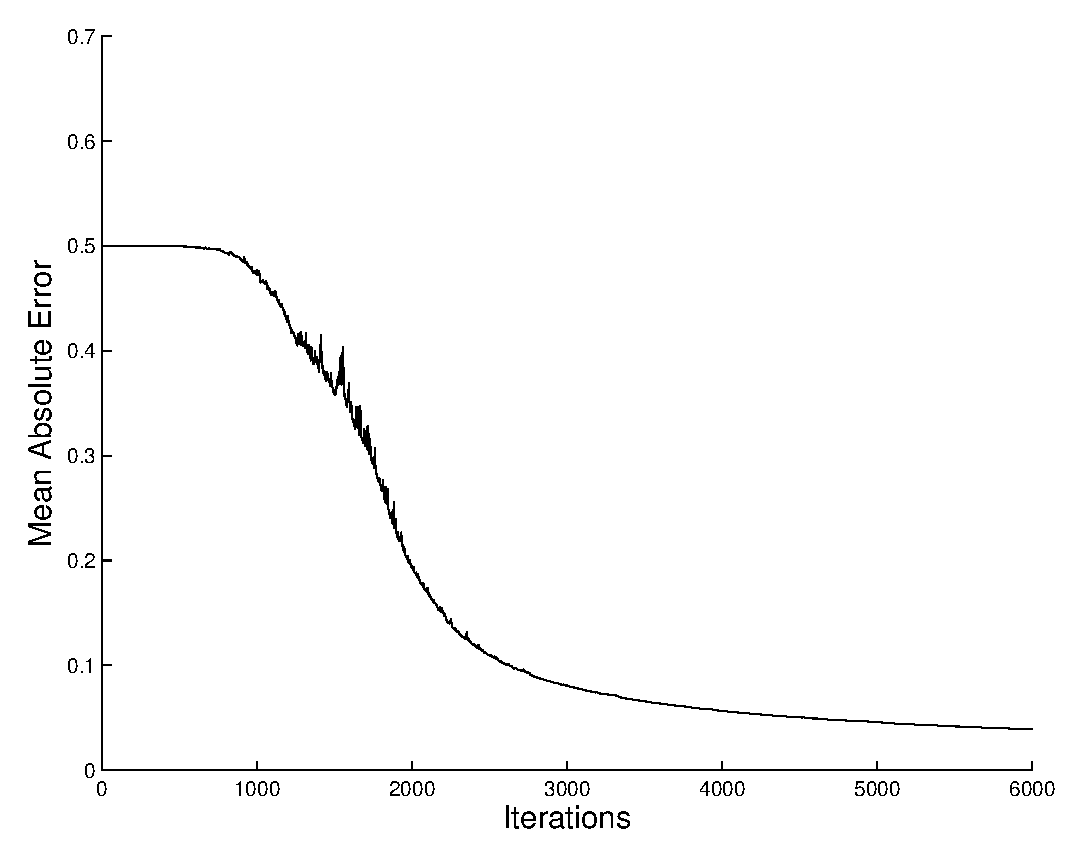
\includegraphics[scale=0.75]{task1-xor-error-6k.eps}
      \caption{Fehlerverlauf für XOR, Lernrate 1}
	  \end{subfigure}
	\end{figure}
	\begin{figure}[H]
	  \begin{subfigure}
	    \centering
	    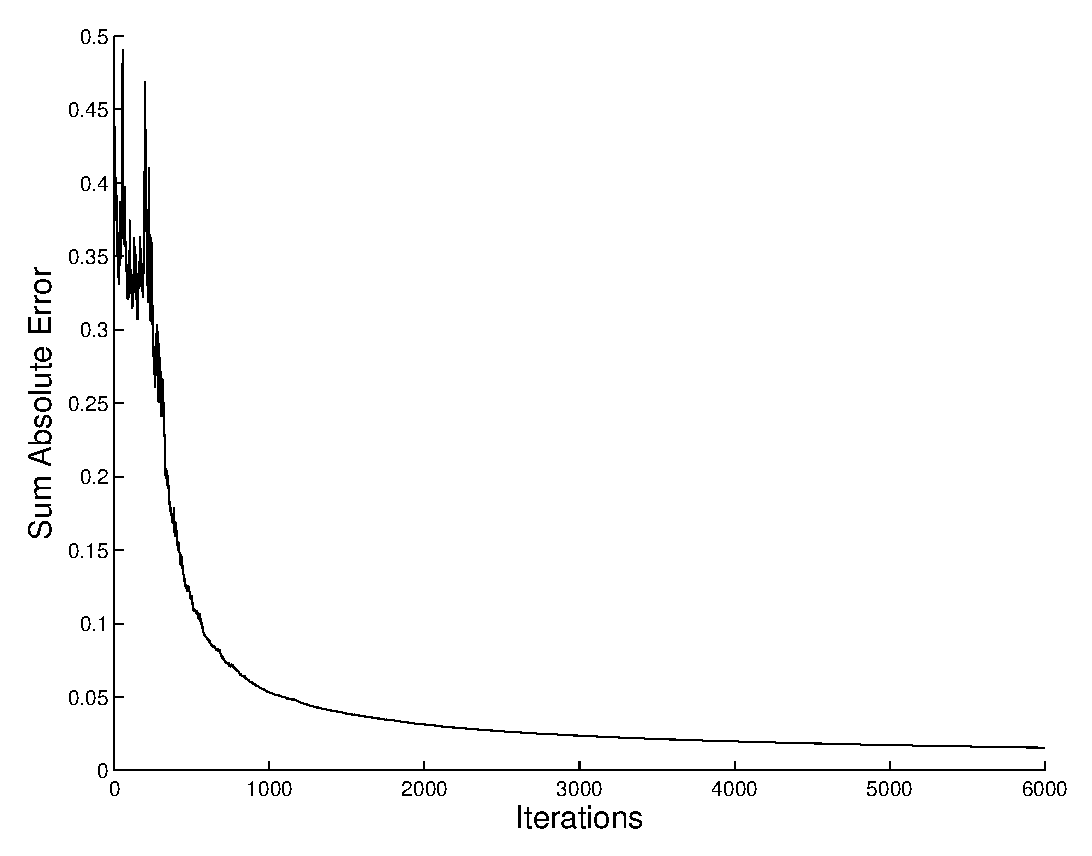
\includegraphics[scale=0.75]{task1-or-error-6k.eps}
      \caption{Fehlerverlauf für OR, Lernrate 1}
	  \end{subfigure}
	\end{figure}
	\begin{figure}[H]
	  \begin{subfigure}
	    \centering
	    \includegraphics[scale=0.75]{task1-and-error-6k.eps}
      \caption{Fehlerverlauf für AND, Lernrate 1}
	  \end{subfigure}
	\end{figure}


\subsection*{2. Pendigits}
  Wir wenden zuerst PCA auf die Daten an und rufen dann wieder unsere generische Backpropagation-Learning Funktion auf.\\
  \begin{lstlisting}
  % -------
  % TASK 2 - Learn Pendigits
  % -------
  tra = load('pendigits.tra');
  tes = load('pendigits.tes');
  %fid = fopen('task1-results.txt','w');
  
  % We standardize the data to adjust for large differences in absolute
  % feature values
  traX = standardize(tra(:,1:end-1));
  traY = toDummyVariables(tra(:,end));  % We need output as dummy variable now
  tesX = standardize(tes(:,1:end-1));
  tesY = toDummyVariables(tes(:,end));
  
  % PCA
  pcs = principalComponents(traX);
  traX = transformData(pcs, traX, 14);
  tesX = transformData(pcs, tesX, 14);
  Ntra = size(traX, 1);
  Ntes = size(tesX, 1);
  
  % Neural Network Training
  K = 15;  % Hidden nodes
  M = 10;  % Output nodes
  learnFactor = 1;  % Learning rate
  maxIterations = 10000001;
  errEvery = 1000000;
  [W1d W2d Eabs Esq Eonline] = learnNeural(traX, traY, K, M, ...
      learnFactor, maxIterations, errEvery);
  EabsMean = Eabs./Ntra;
  EsqMean = Esq./Ntra;
  plotErrorForIterations([([0:size(Eabs,1)-1]*errEvery)' EabsMean], ...
      'task2-abs-err', 'Iterations','Mean Absolute Error');
  plotErrorForIterations([([0:size(Esq,1)-1]*errEvery)' EsqMean], ...
      'task2-sq-err', 'Iterations','Half squared Error');
  plotErrorForIterations([([0:size(Esq,1)-1]*errEvery)' sum(EsqMean,2)/M ], ...
      'task2-sq-mean-err', 'Iterations','Mean half squared Error');
  plotErrorForIterations([([0:size(Eonline,1)-1])' Eonline ], ...
      'task2-sq-mean-err-online', 'Iterations','Mean half squared online Error');
  
  % Test
  tesXd = [tesX, ones(Ntes, 1)];  % convenience
  isVsShould = zeros(Ntes,2);
  for i = 1:size(tesX,1)
    [value index] = max(tesY(i,:));
    realClass = index - 1;
    ourClass = classifyNeural(W1d, W2d, tesXd(i,:));
    isVsShould(i,:) = [ourClass realClass];
  end
  diff = isVsShould(:,1) - isVsShould(:,2);
  right = size(diff(diff==0));
  SuccessRate = right / size(diff)
  \end{lstlisting}
  
  	Wir haben ein paar Experimente durchgeführt und mit den Testdaten evaluiert:
	\begin{table}[H]
	    \begin{tabular}{|l|l|l|l|l|l|l|l|l|l|l|}
	        \hline
         Erkennungsrate & Iterationen & Lernrate \\ \hline
         $ 38.25\% $ & 100 & 1\\
         $ 70.3\% $ & 500 & 1\\
         $ 80.05\% $ & 1.000 & 1\\
         $ 17.55\% $ & 1.000 & $ 0.1 $\\
         $ 88.51\% $ & 10.000 & 1\\
         $ 91.37\% $ & 100.000 & 1\\
         $ 90.11\% $ & 1.000.000 & 1\\
         $ 91.19\% $ & 1.000.000 & $ 0.1 $\\
         $ 91.45\% $ & 1.000.000 & $ 0.01 $\\
         $ 91.94\% $ & 10.000.000 & $ 0.05 $\\
	        \hline
	    \end{tabular}
	\end{table}
	Wir sehen: Am Anfang verhilft eine große Lernrate zu schnellem Lernen.
	Bei vielen Iterationen bringt eine kleine Lernrate jedoch bessere Resultate.\\
	
	Im folgenden die Darstellung des quadratische Fehler, für den der Algorithmus optimiert. Dieser gilt jeweils nur für das aktuelle zufällige Sample und ist daher sehr sprunghaft
	\begin{figure}[H]
	  \begin{subfigure}
	    \centering
	    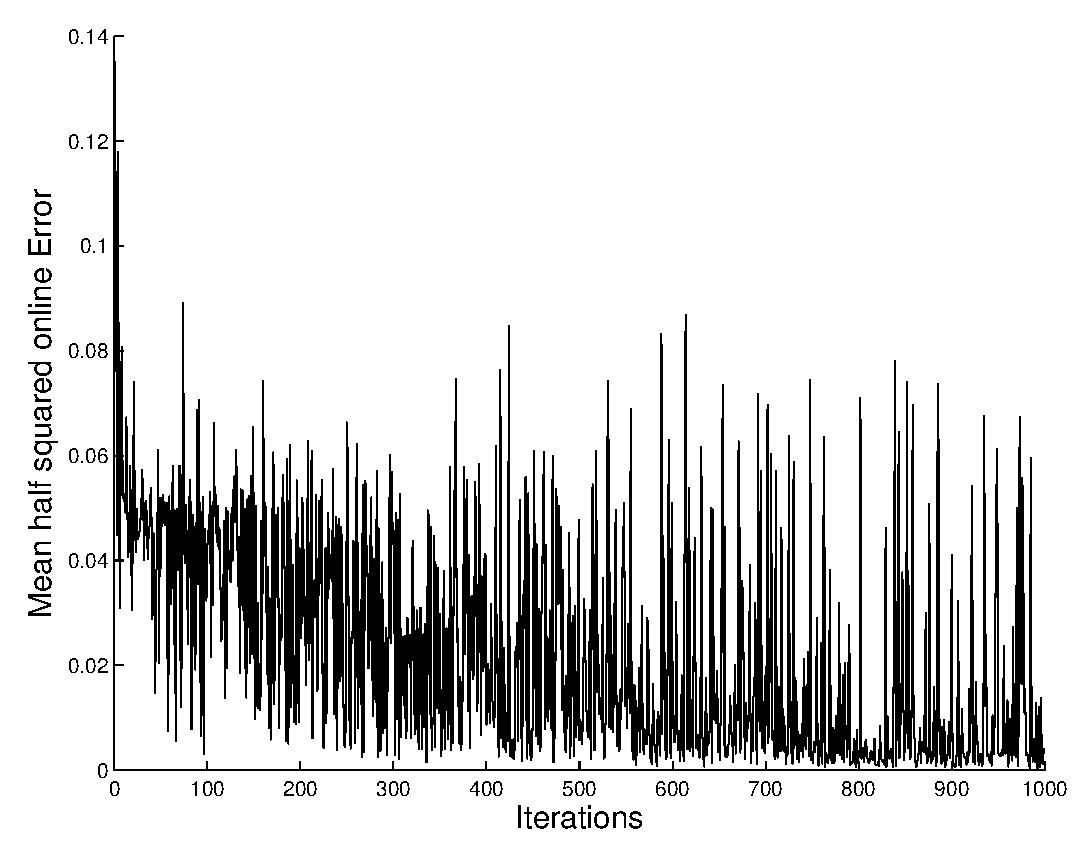
\includegraphics[scale=0.75]{lr100_1K/task2-sq-mean-err-online.eps}
	  \end{subfigure}
	\end{figure}
	
	Nun der selbe quadratische Fehler, jedoch für alle Samples berechnet und gemittelt:
	\begin{figure}[H]
	  \begin{subfigure}
	    \centering
	    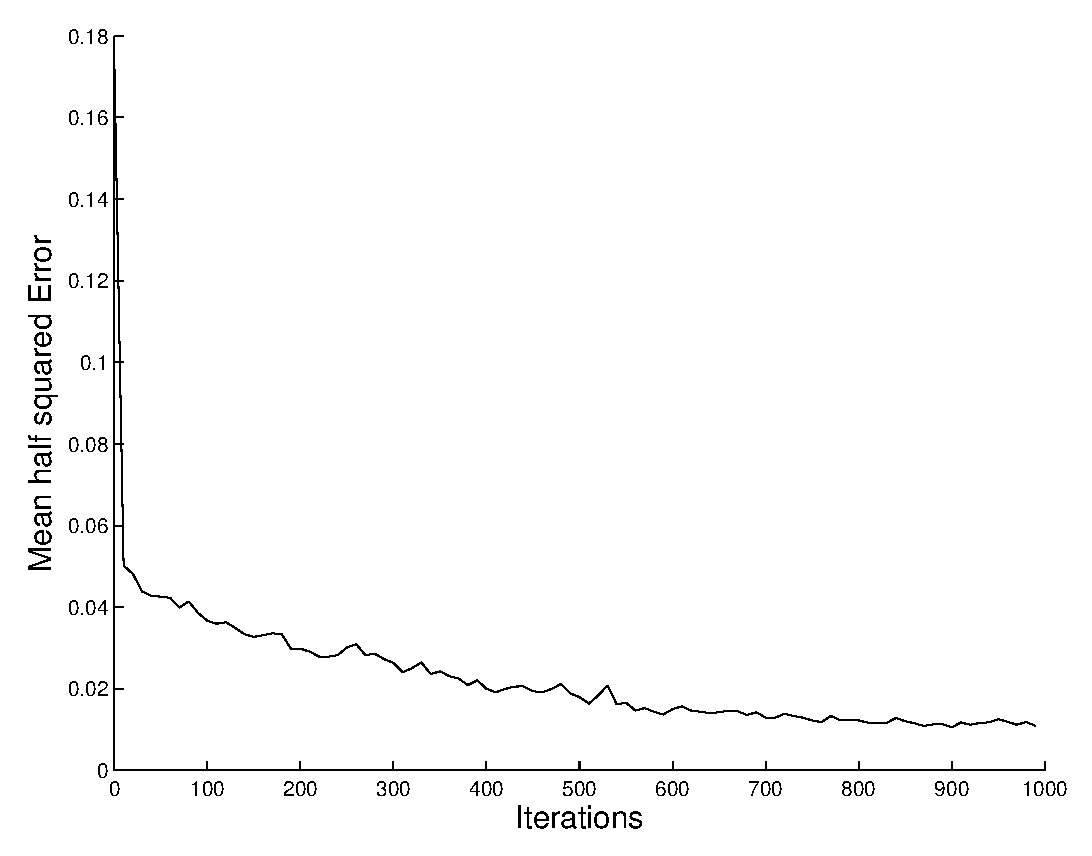
\includegraphics[scale=0.75]{lr100_1K/task2-sq-mean-err.eps}
	  \end{subfigure}
	\end{figure}
	
	Nun die gemittelte absolute Abweichung für alle Samples und die jeweiligen Output-Units:
	\begin{figure}[H]
	  \begin{subfigure}
	    \centering
	    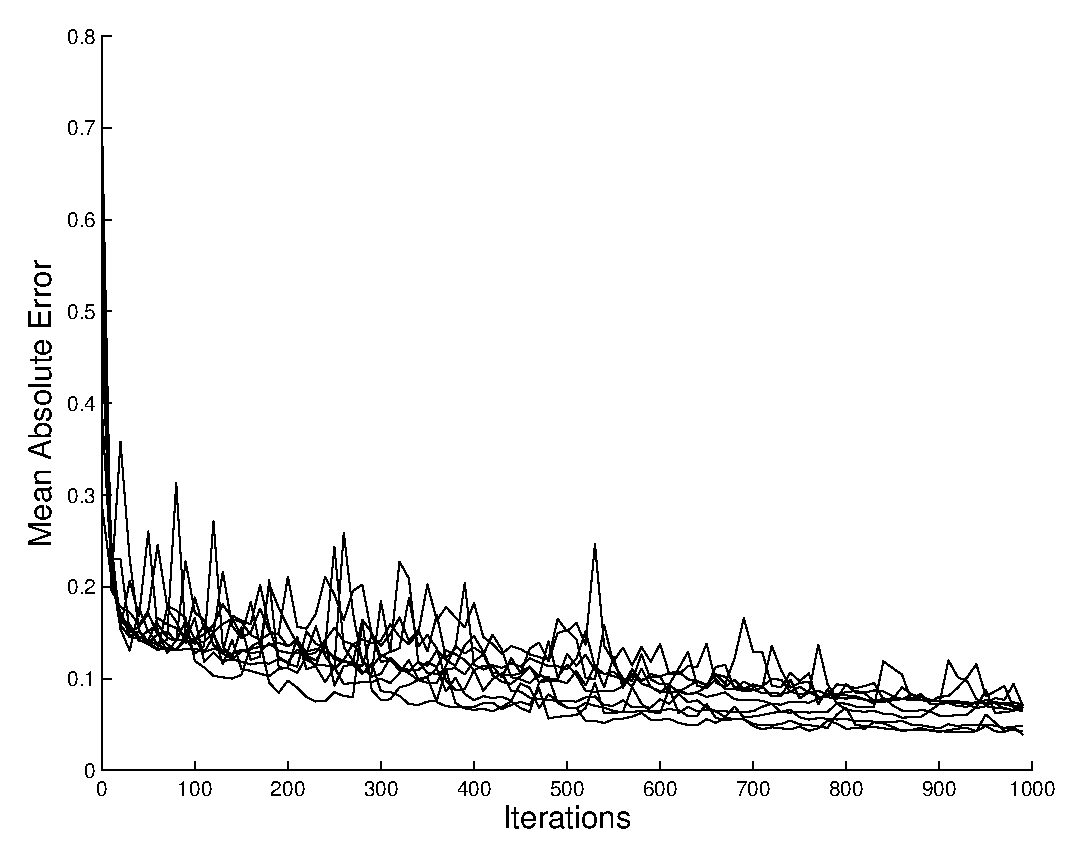
\includegraphics[scale=0.75]{lr100_1K/task2-abs-err.eps}
	  \end{subfigure}
	\end{figure}
  
  Nun noch Experimente mit einer anderen Anzahl von Hidden Nodes:\\
  Lernrate 1, 10 Hidden Nodes, 100.000 Iterationen: $ 88.82 $\\
  Lernrate 1, 15 Hidden Nodes, 100.000 Iterationen: $ 91.17 $\\
  Lernrate 1, 20 Hidden Nodes, 100.000 Iterationen: $ 92.42 $\\
  Lernrate 1, 50 Hidden Nodes, 100.000 Iterationen: $ 92.11 $\\
  Lernrate 1, 100 Hidden Nodes, 100.000 Iterationen: $ 91.82 $\\
  
  Wir sehen dass etwas mehr Hidden Nodes zu besseren Erkennungsraten führen.
  
\end{document}
